\documentclass[04_projectProcess.tex]{subfiles}
\begin{document}
    \subsection{Related Work and Inspiration}
        \begin{flushleft}
            Many products are related to this project. Some of them just have one 
            feature and others have multiple and people use an additional device to handle all 
            the functions.
            
            One product that deals with light are common lights. It is less expensive and 
            only has one function, on or off. Still, nearly anyone has such a lamp in the office. \\

            The number of functions of these lamps is limited. That's why companies 
            gave them additional functions like changing the color. Usually, this can be done 
            by a smartphone app. There, people can define the color of the room. Furthermore, 
            a specific time for the color change can be defined. A product that can 
            change its color is the Philip Hue lamps \cite{philipHue}. In this ecosystem,
            people can do all this in an app.  \\ 

            Still, there is no lamp you can interact with as you do with this one. Here, it 
            allows you to interact and to engage with the lamp again. Furthermore, there is no 
            need for using an app on the smartphone. So, there is less distraction, and anyone 
            can use it. Older people or very young people have problems using a smartphone. 
            People have to find the right app, have to understand how it works and have to read 
            on a small screen.  \\~\\

            A flexible wood notebook was the inspiration that has been found during the summer
            break. There, the cover of the book was out of wood. If you open it, the back of the
            book lighted up (see Figure \ref{fig:inspirationLightUp}) and by closing it the 
            light switched off (see Figure \ref{fig:inspirationLightOff}). This was the 
            inspiration for the whole idea. 

            \begin{figure}[H]
                \centering
                \begin{subfigure}{.45\textwidth}
                    \centering
                    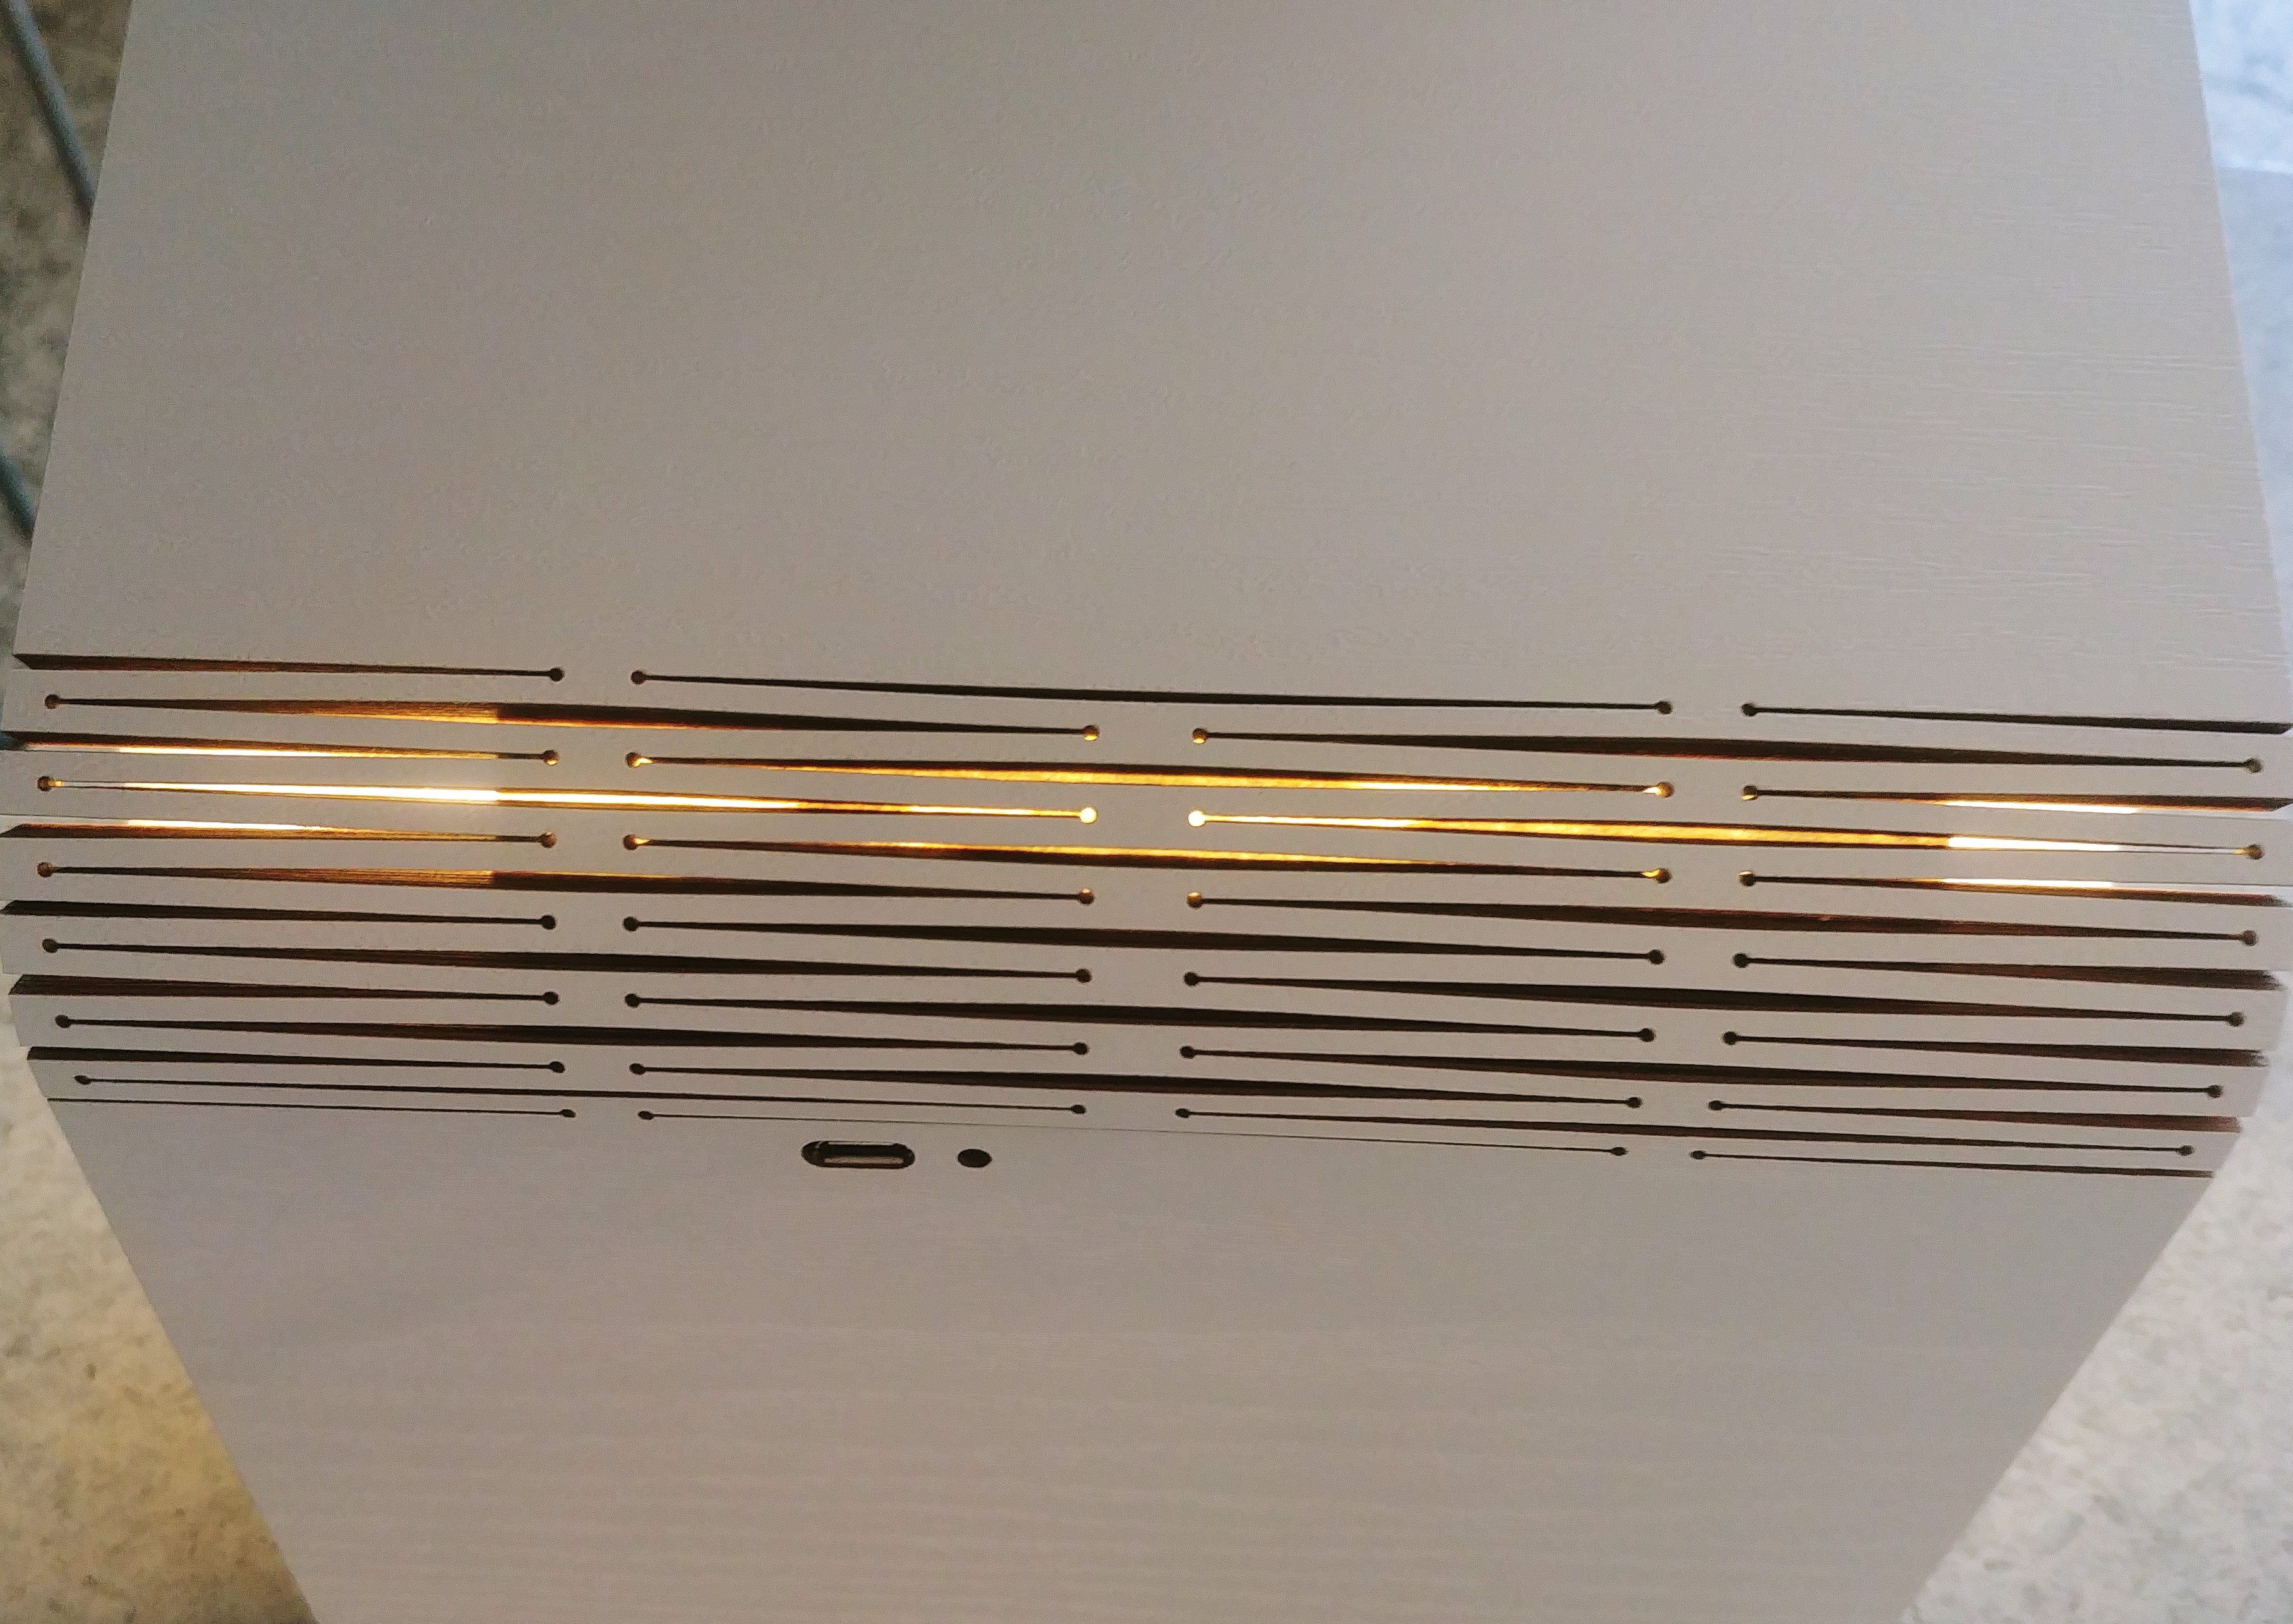
\includegraphics[width=0.8\linewidth]{images/projectideas/inspiration_on.jpg}
                    \caption{Shows the notebook open and light up.}
                    \label{fig:inspirationLightUp}
                \vspace{6mm}
                \end{subfigure}
                \begin{subfigure}{.45\textwidth}
                    \centering
                    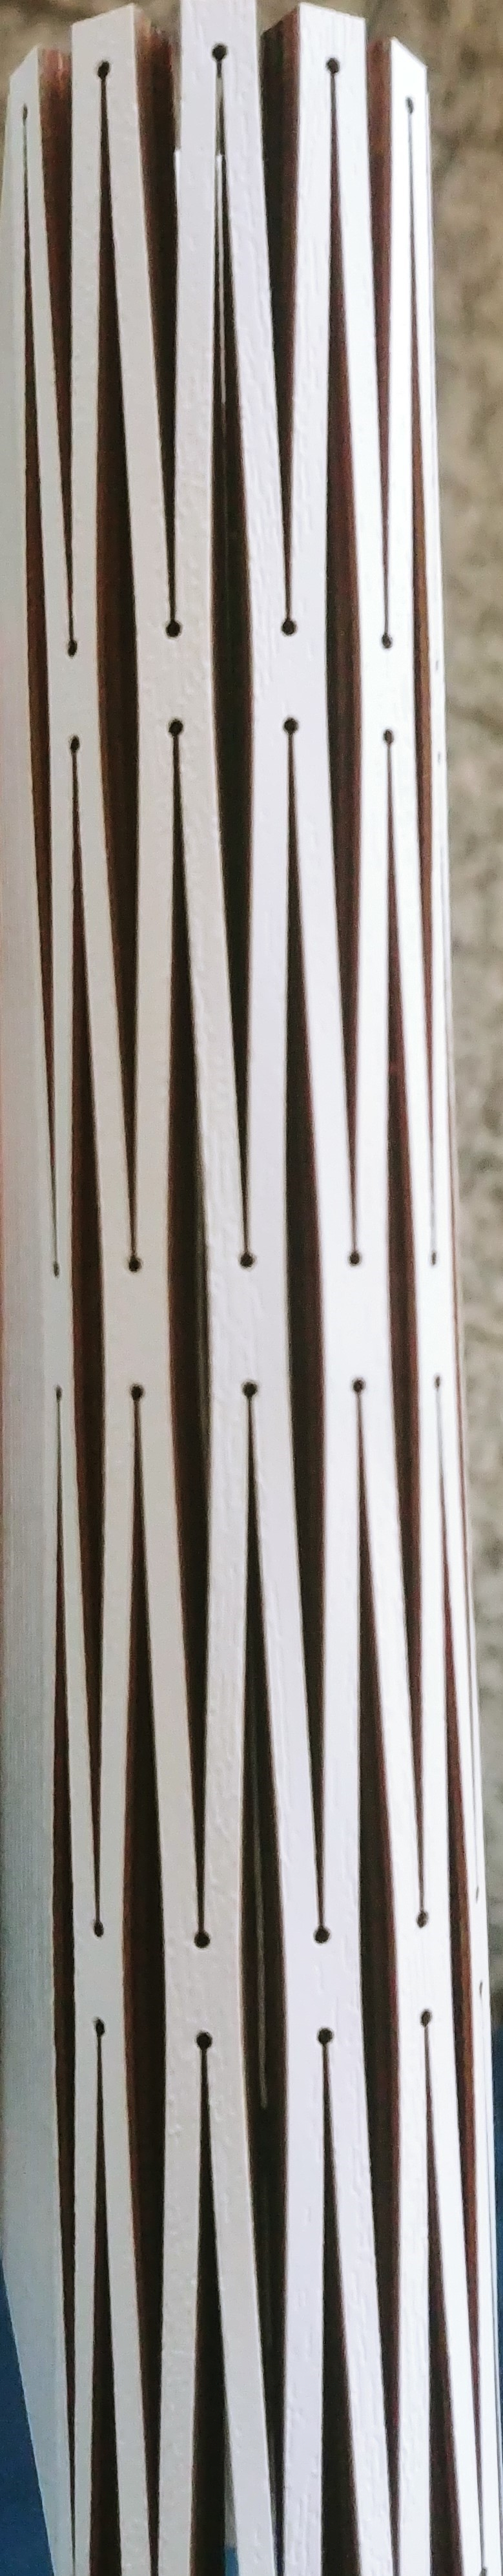
\includegraphics[scale=0.03, angle=90]{images/projectideas/inspiration_off.jpg}
                    \caption{Shows the notebook close and light off.}
                    \label{fig:inspirationLightOff}
                    \vspace{6mm}
                \end{subfigure}
                \caption{Shows the inspiration.}
                \label{fig:inspiration}
            \end{figure}
        \end{flushleft}
\end{document}
